\section{Matériel et méthodes}

\subsection{Besoins fonctionnels principaux}

L'objectif principal est de produire une interface web fonctionnelle pour les outils \textit{Bio++},
et de la deployer sur un serveur du laboratoire d'accueil accessible depuis l'extérieur.
L'interface doit impérativement être simple et accessible pour un publique non-expert,
ciblé essentiellement sur des biologistes travaillant sur des projets en génétique évolutive.
En outre, ce projet permet à un utilisateur potentiel
de s'abstraire de l'installation des différents outils,
qui nécessite une connaissance des environnements Unix-like
leur administration, et la compilation de logiciels C++.
En d'autres termes, l'idée de ce projet
est de permettre de rendre la suite accessible
à un publique beaucoup plus large
en baissant significativement l'effort nécessaire
pour se l'approprier.

Pour ce faire, l'interface doit pouvoir faire l'intermédiaire entre un utilisateur
et la suite \textit{Bio++},
afin de pouvoir spécifier un modèle phylogénétique et rentrer des données,
de façon transparente par rapport à l'implementation des outils.

En effet, la suite d'outils est imposante en premier abord,
nécessitant l'apprentissage d'un langage déclaratif spécifique à \textit{bppsuite},
l'utilisation et le paramètrage des différents logiciels de la suite,
en passant par l'entrée des données et la récupération des sorties,
ainsi que leur interprétation.


\subsection{Considérations additionnelles}

L'interface doit rendre la suite plus attractive à de nouveaux utilisateurs.
Ainsi, sa bonne performance est très importante.
Sa réactivité, efficacité et la rapidité du rendu
doit donc être bien prise en compte dans son design et implémentation.

L'introduction à la suite \textit{Bio++} par le biais de la nouvelle interface
sera facilité par l'accès à des templates de modèles évolutifs,
et un tutoriel rapide,
tous transposés depuis des documents et exemples
déjà disponibles dans les dépôts de \textit{Bio++}.
Leur présence sur l'interface permettra de comprendre par l'exemple
les possibilités de la suite.
Un accès au reste de la documentation déjà générée permettra de plus
à des utilisateurs expérimentés d'aller plus loin dans leurs investigations,
en passant par des modèles de plus en plus complexes.


\subsection{Pipeline basique}

Dans son utilisation la plus basique,
\textit{bppml} prend en entrée une séquence alignée,
un arbre phylogénétique construit au préalable,
et un modèle avec ses paramètres
avec leurs valeurs initiales.
L'arbre est complet et topologique,
et n'est pas optimisé par le logiciel:
c'est le processus évolutif qui l'est.

Les paramètres spécifiés du modèle sont estimés par maximum de vraisemblance
pour inférer le meilleur modèle étant donné l'arbre et les séquences.
Les sorties comprennent les paramètres inférés du modèle,
la meilleure phylogénie reconstruite,
et des fichiers intermédiaires.
Ces fichiers peuvent être réutilisés ensuite
avec d'autres logiciels de la suite \textit{Bio++}
pour d'autres calculs.

La complexité du projet provient du fait que les données d'entrée
peuvent être toutes les combinaisons imaginables
de séquences, de modèles, d'arbres, paramètres ou racines d'arbres,
de nombre différent à chaque fois.
Les modèles peuvent être emboîtés ou réutilisés
dans un autre run de \textit{bppml}.


\subsection{Design}

Pour répondre aux besoins,
le design considéré est celui d'une architecture serveur-client classique.

La partie client sera divisée en deux composantes,
l'une gérant l'entrée et la validation des données et paramètres,
et l'autre le rendu des résultats et leur visualisation.

La partie serveur elle communiquera avec le client
pour générer les lignes de commandes et fichiers d'entrée
pour lancer \textit{bppml},
puis renvoyer les résultats du calcul à l'utilisateur.

Le déployement de l'outil devra être facile et rapide
pour prendre en compte des changements de serveur
ou d'organisation du système de fichiers différente dans l'avenir.
Sa prise en charge par une autre équipe après le terme du projet
doit être sans effort.
Les dépendances du projet doivent donc en outre
être faciles à gérer.
L'implémentation ne doit pas utiliser des chemins en dur sur le système de fichiers
et utiliser des fichiers de configuration
pour s'abstraire de sa localisation.

En termes de performance,
le temps de réponse du serveur doit être minimale,
sans temps de latence supplémentaire par rapport au temps de calcul de la suite.
De l'autre côté, la partie client doit être peu lourde
pour conserver une rapidité même sur des ordinateurs peu puissants,
ce qui est le cas assez fréquemment.

La suite \textit{bppml} peut prendre en charge
des types de données multiples, un ou plusieurs sous-modèles,
avec potentiellement des paramètres différents,
et une multitude de combinaisons
qui rend le nombre de possibilités rapidement ingérable.
Le programme initial sera donc très simple mais modulaire et extensible,
pour implémenter les fonctionnalités basiques,
qui vont soutenir le reste de l'interface,
très rapidement.
Au début, l'interface ne gérera que
des combinaisons d'entrées et de modèles très simples,
puis de plus en plus de possibilités seront ajoutées de façon itérative.
Ceci permettra
de tester facilement au fur et à mesure les nouvelles fonctionnalités,
de permettre de limiter l'implémentation dans le cadre de ce projet
aux fonctionnalités principales,
de donner la capabilité d'ajouter le reste par la suite,
et de s'adapter à l'évolution future de la suite.


\subsection{Implementation}

L'interface sera basée sur une installation de Linux,
adaptée au serveur disponible hébergé par le laboratoire d'accueil.

Les données d'entrée sont une ou plusieurs séquences nucléiques,
un ou plusieurs arbres phylogénétiques élaborés précedemment,
\textbf{et autres}.
Les séquences sont assumées propres et alignées au préalable.
A terme, l'outil saura gérer des alphabets autres
(protéique, codons, etc.),
voire même les mélanger.

\textbf{cf notes: i/o}

Le paramétrage se fera en commençant par un modèle bare-bones,
ou un template de modèle existant,
par le biais de boutons et de menus déroulants
pour rajouter de plus en plus d'éléments au modèle
en fonction des besoins.
Le modèle courant sera visualisé sur un graphe acyclique dirigé,
sur lequel des éléments pourront directement être ajoutés,
copiés, masqués, etc.
\textbf{interface principal = DAG?}

Les sorties seront une phylogénie optimisée
et des visualisations.

Les logiciels ne dépendent pas de données volumineuses
ou de connection à une base de données,
donc la gestion de l'espace de disque dur ne sera pas conséquente.
Par contre, \textit{bppml} peuvent,
pour des modèles relativement complexes,
prendre beaucoup de temps de calcul.
Les résultats devront ainsi potentiellement
être rendus en différé,
par exemple par notification par e-mail,
et en fournissant un lien unique vers eux.

Le serveur peut être implémenté sous Python avec Flask.

Le client utilisera Typescript transpilé en javascript.
Les sorties sont attendues à être assez simples,
pour ne nécessiter que des visualisations relativement simples
sur graphiques SVG générées par D3.js.
Une implémentation single-page est souhaitée.

L'aspect visuel sera géré par des fichiers CSS.

Les pages exposées à l'utilisateur seront clairement documentées,
soit sur une page dédiée,
soit directement et de façon non-intrusive sur l'interface.
De plus, des tool-tips sur les différentes parties de l'interface
la rendront plus facilement utilisable.
Une page indiquera les auteurs, des contacts,
des liens vers les dépôt et leur site officiel,
et les articles de recherche sur la suite.

\textbf{cf notes: détails d'implementation}

Le développement se fera en local sur machine personnelles
avant de le déployer pour qu'il soit accessible publiquement,
pour avoir directement un site fonctionnel dès publication.

\begin{figure}
	\caption{Design général de \textit{bpp-web}}
	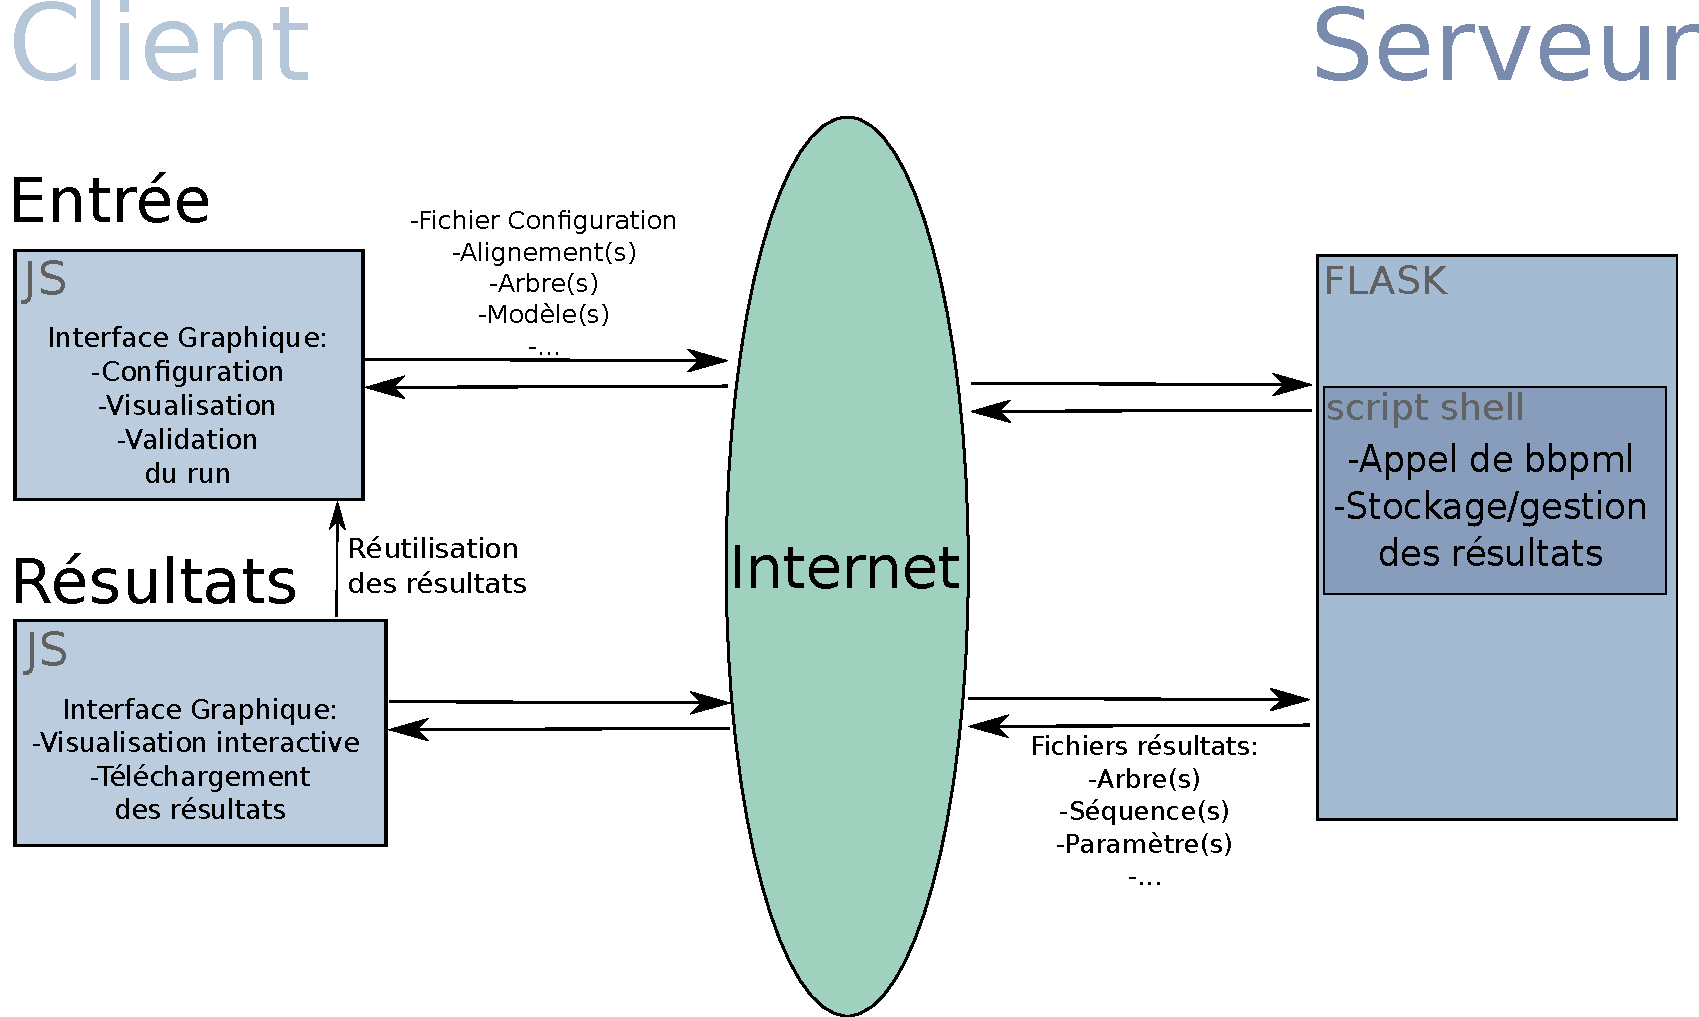
\includegraphics[scale=0.5]{fig/SchemaConcept.pdf}
	\centering
\end{figure}



\subsection{Extensions possibles}

L'interface sera implémentée en français durant le projet,
mais à terme, elle devrait être en anglais d'abord,
avec une option pour la traduire en français.

La fonctionnalité de l'interface est primordiale,
mais un travail sur son aspect visuel est souhaitable également.
